\section{Development Plan}

The success of the \grackle{} project as a community resource will
depend on its ability to adapt to the evolving scientific and
technical needs of the users. Key to this are 1) adding features
desired by users, 2) encouraging external contribution by ensuring
that the code is easily extendable, and 3) improving performance to
keep up with advances in the simulation codes that use it.
The proposed work plan, detailed below, will address each of these key
factors. Each year of the work plan has milestones in the form of
deliverables to the community which will enable specific scientific
goals. The features and improvements that we will implement were all
identified in a \grackle{} user survey carried out in Spring 2017 as
being important to the community. In addition, we identify scientific
collaborators with stated intentions of making use of the new features
developed. Figure \ref{fig:gantt} displays the timeline for the
design, implementation, and delivery of each of the milestones in this
CSSI proposal. \grackle{} and \dengo{} are both distributed under the
3-clause, revised BSD license and have no proprietary dependencies.

\begin{figure}
\begin{center}
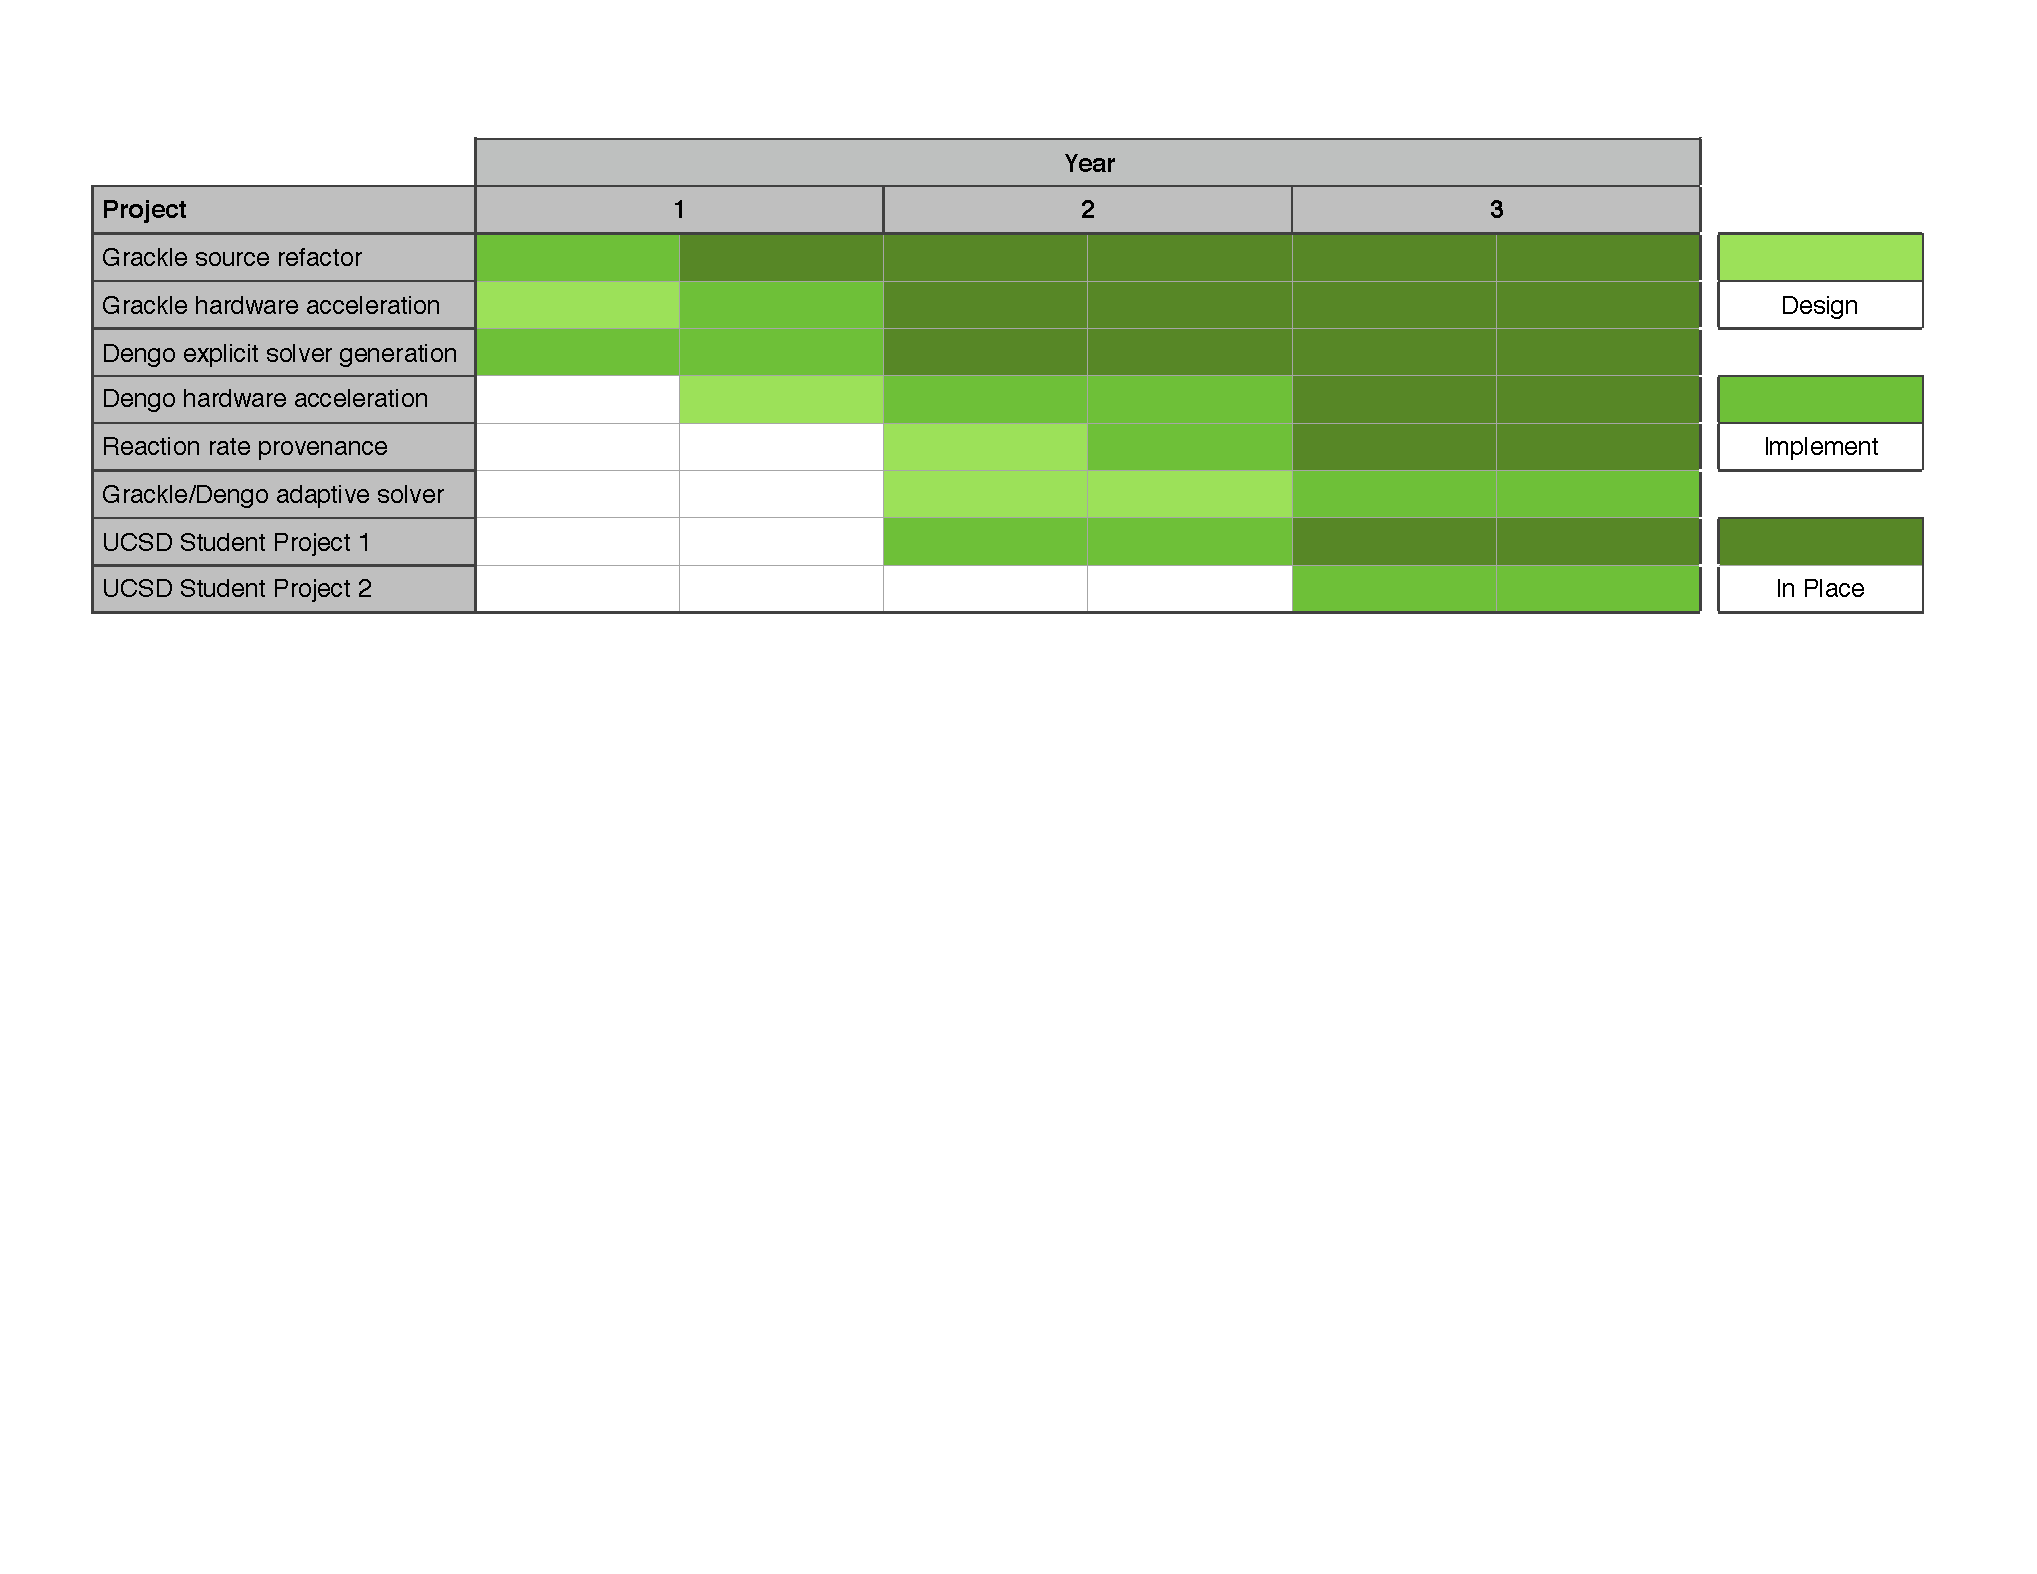
\includegraphics[width=0.7\textwidth]{figures/gantt.pdf}
\caption{Timeline of design, implementation, and delivery of the
  proposed development.}
\label{fig:gantt}
\end{center}
\vspace*{-2\baselineskip}
\end{figure}

\subsection{Year One: Infrastructure Refactor}

The primary goal of the year one development project is to make the
source code substantially more inviting to new contributors and to
build the groundwork for the later projects.  There will be two phases
to this project: 1) expanding the test suite, and 2) porting all
Fortran routines to C.  The planning and commencement of this work
will include direct communication with the \grackle{} user community
via the project's mailing list.  Completion of these phases will be
marked by stable releases.

The design and optimization of the core chemistry and cooling solver
routines in \grackle{} are central factors in making the library fast
enough to be used in extremely large simulations.  However, these
factors also make this the most challenging area of \grackle{} to
work with as a developer.  For example, because there is no simple way
of sharing common/global data or variables between the C and Fortran
routines, the Fortran routines must be handed all parameters, fields,
and rate data as individual arguments.  This results in intimidating
function signatures with dozens of arguments and is only made worse by
the lack of consistency checking between the C and Fortran argument
lists during compilation.  Inconsistencies will result in segmentation
faults whose debugging requires comparison of long lists of function
arguments.  Additional difficulties also include maintaining
consistency in variable type across the C/Fortran interface and the
general confusion that can arise from working in two different
languages at once.  These factors increase the likelihood of bugs and
make the source code significantly less inviting for new
contributors.

The primary advantage of using Fortran for \grackle{}'s most
computationally expensive routines is the speed of array operations.
This is extremely important for \grackle{}, as the code is designed to
work on multiple, large arrays of fields.  This speed advantage was
especially great when the core solvers were originally developed in
the mid-1990s.  However, since that time, advances in the C
programming language, such as the \texttt{restrict} keyword introduced
in the C99 standard \citep{c99}, have made it possible for C code to
be competitive with Fortran.

Phase 1 of the infrastructure refactor will be an expansion of the
test suite to ensure that all functionality and parameter
combinations are covered by answer and unit tests.  The current
test suite adequately covers the most common running modes of the
library, but is insufficient for a full overhaul such as what will
follow.  The completion of phase 1 will be marked by
the release a new stable version of the library.  At the time of
writing, the latest stable release of \grackle{} is version 3.0 with a
3.1 release likely to occur in the next month to cover new features
and bugfixes.  As phase 1 would constitute no change in the library
itself, the resulting release will be a 3.x version (i.e., 3.2 if the
prior version is 3.1).

With a more robust test suite in place, the Fortran code (roughly 7200
lines) can be safely ported to C (phase 2).  The resulting code will
be vastly streamlined as it will no longer be necessary to pass all
required data via function argument.  Instead, the central routines
will be able to access the C \texttt{structs} containing the run-time
parameters, rate data, and field arrays.  In addition, the ease of
calling C routines from Python will allow for the addition of
finer-grained unit tests operating within the existing test suite,
which uses the \texttt{pytest} Python package.  This will also allow
for more of the core functionality to be exposed directly to the user,
as has often been requested.
At present, on startup \grackle{} computes lookup tables from the
functional forms of the reaction rate coefficients.  To enable easier
selection, and greater provenance tracking, we will enable the
\texttt{pygrackle} wrappers to generate pre-computed tables from
functional forms defined in yaml files.  This will provide a method of
experimenting with different rates, such as from different
experimental results or theoretical calculations, while avoiding the
complexity of code generation or full recompilation of the
application.  Finally, with this refactor, the
increased modularity will allow for the implementation of different
solver methodologies.  One potential application of this could be the
fully-implicit solver LSODE \citep{LSODE}.  While LSODE is much slower in many
cases, it allows the individual to specify a more strict convergence
criteria and error threshold than the existing method in \grackle{}.
This may provide utility for situations where \grackle{} struggles
with time-step convergence, such as at extremely high densities.
The result of phase 2 will be a streamlined, more flexible,
refactored source code that will be substantially easier to develop
and will be released as \grackle{} version 4.0.

\textbf{Science Enabled:}

\subsection{Year Two: Hardware Acceleration}

In order for \grackle{} to continue to be a valuable software element
for the astrophysical community, use of the library must not become
the limiting factor for scaling up simulations.  Because the
calculations performed by \grackle{} are all local to each fluid
element (i.e., solving a given cell does not require information about
neighboring cells), it was straightforward to achieve modest speedup
with OpenMP simply by threading the outer loops for which the core
functions are called.  However, significantly greater speedups can be
achieved by parallelizing the operations within the solvers and taking
advantage of hardware acceleration options currently available on the
latest high performance computing (HPC) systems, such as graphics
processing units (GPUs) and many integrated core architectures (MICs).
For example, \citet{Haidar2016PerformanceAA} report speedups of a
factor of 20-40
for an explicit chemistry network ported to a GPU and even greater
speedups when the GPU is used to compute multiple networks
simultaneously.

National computing facilities used for astrophysical simulations, such
as those in the Extreme Science and Engineering Discovery Environment
(XSEDE) and NCSA Blue Waters, employ acceleration with both GPUs and
MIC architectures.  Implementing separate parallelization strategies,
while potentially resulting in faster code, will likely make the
source code more difficult to work with for new developers.  Instead,
we will develop a new parallelism strategy using the OpenACC standard,
which works with many different architectures.  OpenACC is supported
by PGI, Cray, and GNU compilers.  Similar to OpenMP, OpenACC provides
compiler directives, or pragmas, that allow the programmer to
designate portions of code, particularly loops, to be run on the
accelerator.  Additional directives provide control of when data is
copied to and from the accelerator and also to allow certain data to
exist only in the accelerator's memory.  This strategy is well-suited
to \grackle{}'s core functions which make use of a number of temporary
variables and data to perform many operations on a series of input
arrays.

Adding OpenACC support will happen in year two.  The strategy will be
mapped out in year one during the infrastructure refactor.  We will
make use of local computing resources at the PI's home institution
(San Diego Supercomputer Center, SDSC) for development and testing.
SDSC's Comet supercomputer has 36 NVIDIA dual K80 nodes and 36 NVIDIA
4-way P100 nodes.  SDSC is also an Intel Center of Excellence, hosting
a small Knights Landing (KNL) cluster which will be used for testing
on MIC architectures.
We will also work with system administrators at XSEDE facilities to
provide modules of pre-built \grackle{} libraries to users.  When this
project is completed, we will
release version 5.0 of the \grackle{} library.  Included in this
release will be documentation aimed at new developers with
instructions for parallelizing new features.  To support the broader
impacts of this effort, we will also host a
workshop at UCSD at the end of year two to provide instruction and
a venue for collaboration to researchers interested in contributing
new features.

\textbf{Science Enabled:}

\subsection{Year Three: Feature Expansion}

The goal of the year three development project is to expand the user
base of \grackle{} to include the present-day star formation
community.  
In contrast to the early Universe, where only H$_{2}$ is important,
star forming clouds in the local Universe are governed by a host of
additional processes, including heat input from cosmic rays and nearby
stars; cooling from molecules like CO, OH, and H$_{2}$O; cooling from
atomic C/O fine-structure emission; and both heating and cooling
effects from dust grains.  Following the detailed chemical structure
of these complex environments is currently outside the range of
\grackle{}'s capabilities.  However, detailed studies of the minimal
chemistry networks required for accurately modeling these systems
\citep{2012MNRAS.421..116G, 2017ApJ...843...38G} have paved the way
forward.  Expanding the chemistry solver to include additional species
will help to significantly grow the community of \grackle{} users.
This expansion was also the number one requested feature (by 16 out of
23 total respondents, representing 9 of the supported codes) in a
recent online survey of current \grackle{} users.

In year three, the existing primordial chemistry network will be
expanded to include the network of \citet{2017ApJ...843...38G}.  This
is an 18-species network that includes O, O$^{+}$, C, C$^{+}$, CO,
HCO$^{+}$, Si, Si$^{}$+, CH$_{x}$ and OH$_{x}$ (CH$_{x}$ and OH$_{x}$
are pseudo-molecules representing multiple molecules) in addition to
the species currently covered by \grackle{}.
\citet{2017ApJ...843...38G} show that this network out-performs all of
the minimal models discussed in \citep{2012MNRAS.421..116G} when
compared to the results of a more sophisticated photo-dissociation
region calculation.  The improvements made in years one and two will
make this effort significantly easier than if it were undertaken
first.  This will also provide a clear path for implementation of
additional networks in the future.  The year three project both adds
functionality and provides a template for user contributions.

This model will be added to \grackle{} using the parallelization
strategy implemented in year two and will be released as a 5.x version
of the \grackle{} library.

\subsection{Engineering and Release Process}

The \grackle{} project follows an established model for development
and releases that is based on other successful community software
projects in which \grackle{}'s developers participate.  The main
source code repository is hosted on
BitBucket.org\footnote{\url{https://bitbucket.org/grackle/grackle}}
and is publicly readable.  Development proceeds via a ``Pull Request''
model that allows for incoming changes to be effectively peer-reviewed
before  being accepted into the main branch.  The \grackle{} library
uses semantic versioning and
is released with numeric versions in an X.Y.Z format, e.g. ``version
2.3.1''.  Changes to the \grackle{} API or a fundamental restructuring
of the source (such as the year one development project) constitute
changes to the X number in a release.  A change in Y occurs when new,
non-API-breaking features are added.  A change in Z marks a release
containing only bugfixes, but no new functionality.

This development process is primarily modelled after that
of the \yt{} community.  The \yt{} project has similar
aims as a cross-platform library for simulations and PI Britton Smith
and Collaborator Matthew Turk have played significant roles in growing
its community and crafting its governance model.  Similar to
\yt{}, the \grackle{} project maintains Community Code of
Conduct and Developer Guide documents to promote a diverse and
inviting community.

\grackle{} is developed using the Mercurial distributed version
control system.  The main repository on BitBucket.org is publicly
readable with write-access currently granted to a handful of the most
experienced developers.  The Pull Request model is used even by those
with write access to the main repo.  In this model, a contributor
``forks'' the main repository, commits changes to their fork, and then
submits a Pull Request allowing other developers to review the
line-by-line changes.  Reviewers leave comments or ``approve'' the
Pull Request and it is eventually accepted or declined in a process
analogous to peer-review for publications.  At the present time, this
usually proceeds with the lead developer (PI Britton Smith) serving as
Pull Request manager by identifying appropriate reviewers (including
himself) and soliciting comments.  As the community continues to grow,
this role can become codified and rotated amongst multiple people.
\grackle{} has received 54 Pull Requests since the first release.

\grackle{} contains a suite of unit and answer
tests that can be run manually using the \texttt{pytest} package.  The
test suite is also run automatically on the central repository and its
forks using the Bitbucket Pipelines continuous integration service.
When a new Pull Request is issued, the results of the test suite are
shown on the Pull Request's web page with links to more detailed
output which can be examined when failures occur.  The test suite
includes a variety of different tests to guard against regression.
Several ``unit tests'' exist to ensure that fundamental
constraints are not violated.  For example, the cooling rates should
match for identical fluid containers that have different internal unit
systems or are in different cosmological reference frames (i.e.,
comoving or proper).  \grackle{} also has a series of ``answer
tests'', wherein the results of specific calculations are compared
against stored values from prior versions.  Finally, to ensure that
the library continues to function as advertised, the test suite
attempts to compile and run the example codes that demonstrate the
APIs.

\grackle{}'s documentation is included in the source and is written in
reStructuredText, which can be converted to HTML and PDF formats
using the Sphinx package.  An HTML rendering of the documentation is
also hosted on
readthedocs.org\footnote{\url{https://grackle.readthedocs.io}},
and is automatically rebuilt when changes are added to the main
repository.

\subsection{Provenance and Reproducibility}

Reproducibility is integral to the scientific process, but can be
difficult to achieve when a calculation relies on a complex software
stack where dependency versions change frequently
\citep{2014arXiv1412.5557J, 2016arXiv161009958L}.  Increased
community involvement in a project, quickening the churn within the
source code, only exacerbates the situation.  In \grackle{}, this
problem is solved by building unique version identifiers directly
into the library.  When the library is compiled, the Mercurial
changeset hash (an effectively unique series of alpha-numeric
characters) is baked into a routine that outputs relevant information
both to a file, called ``GRACKLE\_INFO'', and to the terminal (via
STDOUT) whenever the library's initialize function is called.  In
addition to the changeset hash, the following information is written:
a ``diff'' of any uncommitted changes made to the source, the release
version, all compilation options, and all run-time parameters.
Additionally, \grackle{} maintains a ``CITATION'' file within the
source and in the documentation describing the proper citation
language and BibTex entries to the citable entities.  We will also
follow external examples, where appropriate, to produce machine
readable provenance information \citep[e.g.,][]{force11,
  Fenner097196}.  In these ways, \grackle{} serves as an example to
the community of mechanisms for making reproducibility documents.

\subsection{Alternative Software Packages}

There is a dearth of cross-platform chemistry and cooling packages 
packages available to the astrophysical simulation community.  This
fact was the primary motivator for \grackle{}'s creation.  The main
alternative to \grackle{} is the 
\texttt{KROME}\footnote{\url{http://kromepackage.org/}} package
\citep{2014MNRAS.439.2386G}.  \texttt{KROME} exposes a number of
distinct chemical networks through a Fortran-based API and can also
generate solver code for a custom network defined by the user.
\texttt{KROME} is designed exclusively as a chemistry network solver
and so does not employ cost-saving simplifications, like tabulated
metal cooling and self-shielding models, designed to work in regimes
where direct network solving is computationally prohibitive.
\texttt{KROME}'s solvers are designed to operate on a single fluid
element and do not offer additional parallelization; \texttt{KROME} is
not specifically targeted toward large simulations.

Several other codes exist for solving specific chemistry
networks on single fluid elements, such as 
\texttt{ALCHEMIC} \citep{2010A&A...522A..42S}, \texttt{ASTROCHEM}
\citep{2013MNRAS.431..455K}, \texttt{ASTROCHEM} \citep[][unrelated to
the first \texttt{ASTROCHEM}]{2013A&A...559A..53M}, \texttt{NAHOON}
\citep{2012ApJS..199...21W}, and \texttt{XDELOAD}
\citep{2005Ap&SS.299....1N}.  The \texttt{ASTROCHEM} by
\citet{2013A&A...559A..53M} is the only code hosted in a
publicly-viewable repository.  \texttt{NAHOON} is downloadable as a
static tar file.  \texttt{ALCHEMIC} and \texttt{XDELOAD} are available
upon request.  \texttt{ASTROCHEM} by \citet{2013MNRAS.431..455K} is a
private code.
In addition to the above codes, a number of works have provided tables
of cooling rates \citep{1993ApJS...88..253S, 2009MNRAS.393...99W,
2013MNRAS.434.1043O} that require the surrounding machinery for
interpolating and updating the internal energy to be implemented
independently.
These codes and tables supply important functionality, but it is
not their aim to provide a flexible API to large simulations, nor to
act as a two-way resource that both serves and invites contribution
from the larger community.

The \grackle{} project has focused on providing optimized, easily
adoptable functionality that is independent of simulation code
design.  Through its interoperability with other cross-platform
astrophysical tools like \yt{}, it seeks to exist within the
ecosystem of scientific software rather than alongside it.
Its focus on usability, performance, and community
involvement make it a vital software element to the field of
computational astrophysics.  This focus is underscored by the goals
of the work outlined in this SSE:
to make the source code easier to develop and more inviting to new
contribution; to enhance performance to scale with next-generation
simulations; and to add features that extend the code to new
communities.

\textbf{Science Enabled:}

\subsection{Advisory Board}

We have formed an advisory board to ensure that the milestones
outlined in this SSE are accomplished satisfactorily and in a timely
fashion.  PI Britton Smith will meet regularly (between 1 and 3 times
per year, via video-conference) with the full board to present updates
on technical progress and progress in achieving the overall goals of
the SSE in terms of growth in users and community involvement.  The
advisory board members are experts in the fields of computational
astrophysics and astrochemistry and have significant experience in the
development (both technical and social) of community software projects
and in parallelizing codes for GPUs and MIC architectures.
{\bf Prof. Greg Bryan} is the original author of the \texttt{Enzo}
simulation code and provides experience with chemistry solving methods
and design of large software projects.
{\bf Dr. Anshu Dubey} was an associate director of the Flash Center
for computational science and one of the lead developers of the
\texttt{FLASH} simulation code \citep{2000ApJS..131..273F,
  2009arXiv0903.4875D}.  Dr. Dubey brings expertise in developing
large adaptive mesh-refinement codes and can advise on adding
\grackle{} support to \texttt{FLASH}.
{\bf Dr. Simon Glover} is a foremost expert in astrochemistry and
chemical networks and has contributed numerous updated chemical rates to
\grackle{}.  Dr. Glover will provide expertise in creating chemical
networks and evaluating their scientific applicability.
{\bf Prof. Michael Norman} is the head of the San Diego Supercomputer
Center and has coordinated development of \texttt{Enzo} and
\texttt{CELLO}/\texttt{Enzo-P}, a peta-scale AMR framework and
simulation code.  Prof. Norman provides experience in software design for
high performance computing and accelerating codes with GPUs and MIC
systems.
{\bf Prof. Stella Offner} is an expert in simulations of present-day
star formation and provides insight into the needs of that community.
Prof. Offner will also advise on adding support for \grackle{} to the
\texttt{ORION} simulation code \citep{2012ApJ...745..139L}.
{\bf Prof. Matthew Turk} is the founder of the \yt{} project and
a core developer of the \texttt{Enzo} simulation code, including
components of the chemistry solver that went into \grackle{}.

The advisory board provides a range of scientific and technical
expertise as well as experience with community software development.
Their input will help to see that milestones are met and that
the project satisfies the needs of the communities it seeks to serve.
